% !TEX encoding = UTF-8 Unicode
% ------------------------------------------------------------------------------
% Este fichero es parte de la plantilla LaTeX para la realización de Proyectos
% Final de Grado, protegido bajo los términos de la licencia GFDL.
% Para más información, la licencia completa viene incluida en el
% fichero fdl-1.3.tex

% Copyright (C) 2012 SPI-FM. Universidad de Cádiz
% ------------------------------------------------------------------------------

Este capí­tulo trata sobre todos los aspectos relacionados con la implementación del sistema en código, haciendo uso de un determinado entorno tecnológico.

\section{Entorno de Construcción}\label{sec:entorno-construcción}

Como se ha especificado en la sección \ref{sec:arquitectura-fisica}, el desarrollo de este proyecto ha sido realizado haciendo uso del equipo del propio alumno, sin necesidad de alguna herramienta hardware extra. Para ello, se ha hecho uso de un marco tecnológico específico que se detallará a continuación: 

\paragraph*{Hardware}

Los elementos del hardware utilizados no son relevantes para el desarrollo del sistema, ya que no se requiere nada fuera de lo común en un equipo de trabajo convencional. En este caso, se ha utilizado un portátil MacBook Pro de 15 pulgadas, con procesador Intel Core i7 de 2.2 GHz y memoria RAM de 16GB 1333 MHz DDR3.

\paragraph*{IDE (Entorno de Desarrollo Integrado)}

NetBeans es un IDE libre y gratuito pensado especialmente en desarrollo de software bajo el uso del lenguaje de programación Java.

\paragraph*{Lenguaje de Programación} 

Para la realización de la aplicación web se ha utilizado el lenguaje de programación \textbf{Java}, en concreto la plataforma Java EE (Enterprise Edition), con la ayuda de varios frameworks para diferentes cometidos, como son JSF, PrimeFaces, EJB y JPA, que se describirán a continuación.

\paragraph*{Frameworks}

\begin{itemize}
\item \textbf{JSF (JavaServer Faces):} framework MVC que proporciona un conjunto de componentes en forma de etiquetas definidas en páginas XHTML mediante el framework Facelets. Se utiliza para aplicaciones Java basadas en web simplificando el desarrollo de interfaces de usuario. 
\item \textbf{Facelets:} framework basado que permite definir la estructura general de las páginas (su layout) mediante plantillas. Facelets se adapta perfectamente al enfoque de JSF y se incorpora a la especificación desde la revisión 2.1. Anteriormente, las páginas JSF se definían utilizando etiquetas específicas de JSP, lo que generaba cierta confusión porque se trata de enfoques alternativos para un mismo problema. La sustitución de JSP por Facelets como lenguaje básico para definir la disposición de las páginas permite separar perfectamente las responsabilidades de cada parte del framework. La estructura de la página se define utilizando las etiquetas Facelets y los componentes específicos que deben presentar los datos de la aplicación utilizando etiquetas JSF. Para más información sobre JSF y/o Facelets véase el enlace \ref{bio:introduccion-jsf} de la biografía.
\item \textbf{PrimeFaces:} este framework es una extensión de JSF de código abierto que cuenta con un conjunto de componentes enriquecidos para facilitar la creación de interfaces de usuario.
\item \textbf{EJB (Enterprise JavaBeans):} plataforma para construir aplicaciones empresariales portables, reusables y escalables, utilizando el lenguaje de programación java. EJB permite a los desarrolladores de aplicaciones enfocarse en construir la lógica de negocio sin la necesidad de gastar tiempo en la construcción de código de infraestructura. 
\item \textbf{JPA (Java Persistence API:} La persistencia dentro de EJB es administrada por JPA. JPA permite persistir automáticamente los objetos Java utilizando una técnica denominada object-relational mapping (ORM). ORM es esencialmente el proceso de mapear la información contenida en los objetos Java hacia las tablas de base de datos utilizando una configuración.
JPA define un estándar para:
\begin{itemize}
\item La creación de configuración metadata del ORM para mapear entidades hacia tablas relacionales.
\item La EntityManager API, una API estándar para realizar las operaciones CRUD (create, read, update y delete) de las entidades.
\item El lenguaje Java Persistence Query Language (JPQL), para realizar búsquedas y obtener información persistida de la aplicación.
\end {itemize}
\end {itemize}

En la siguiente figura podemos ver una representación de la integración de los frameworks descritos en la arquitectura de 3 capas vista en la sección \ref{sec:arquitectura-logica}.

\vspace{10mm}

\begin{figure}[H]
\centering
  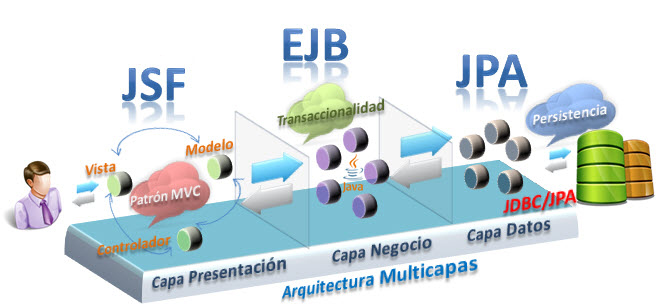
\includegraphics[scale=.75]{img/arquitectura-jee.jpg}
  \caption{Arquitectura de 3 Capas con Frameworks}
  \label{fig:arquitectura-jee}
\end{figure}

\vspace{10mm}

\paragraph*{SGBD}

\paragraph*{Control de Versiones}



\subsection{Entorno para la Web Pública}


En esta sección se debe indicar el marco tecnológico utilizado para la construcción del sistema: entorno de desarrollo (IDE), lenguaje de programación, herramientas de ayuda a la construcción y despliegue, control de versiones, repositorio de componentes, integración contí­nua, etc.



\section{Código Fuente}
Organización del código fuente, describiendo la utilidad de los diferentes ficheros y su distribución en paquetes o directorios. Asimismo, se incluirá algún extracto significativo de código fuente que sea de interés para ilustrar algún algoritmo o funcionalidad especí­fica del sistema.

\section{Scripts de Base de Datos}
Organización del código fuente, describiendo la utilidad de los diferentes ficheros y su distribución en paquetes o directorios. Asimismo, se incluirá el script de algún disparador o un procedimiento almacenado, que sea de interés para ilustrar algún aspecto concreto de la gestión de la base de datos.
